\section{3D Geometric Transformations}

\subsection{3D Translation}

$$
\begin{aligned}
  P^\prime &= T \cdot P \\
  \begin{bmatrix}
    x^\prime \\
    y^\prime \\
    z^\prime \\
    1
  \end{bmatrix}
  &=
  \begin{bmatrix}
    1 & 0 & 0 & t_x \\
    0 & 1 & 0 & t_y \\
    0 & 0 & 1 & t_z \\
    0 & 0 & 0 & 1
  \end{bmatrix}
  \begin{bmatrix}
    x \\
    y \\
    z \\
    1
  \end{bmatrix}
\end{aligned}
$$

\subsection{3D Coordinate-Axis Rotation}

어떤 좌표축을 중심축으로 회전하는 경우. 3차원 회전은 축이 적어도 3개 이상이다. 이때 중심축이란 회전하지 않는 점이 있는 축.

\subsubsection{z-axis Rotation}

$$
\begin{aligned}
  P^\prime &= R_z(\theta) \cdot P \\
  \begin{bmatrix}
    x^\prime \\
    y^\prime \\
    z^\prime \\
    1
  \end{bmatrix}
  &=
  \begin{bmatrix}
    \cos \theta & -\sin \theta & 0 & 0 \\
    \sin \theta & \cos \theta & 0 & 0 \\
    0 & 0 & 1 & 0 \\
    0 & 0 & 0 & 1
  \end{bmatrix}
  \begin{bmatrix}
    x \\
    y \\
    z \\
    1
  \end{bmatrix}
\end{aligned}
$$

\subsubsection{x-axis Rotation}

$$
\begin{aligned}
  P^\prime &= R_x(\theta) \cdot P \\
  \begin{bmatrix}
    x^\prime \\
    y^\prime \\
    z^\prime \\
    1
  \end{bmatrix}
  &=
  \begin{bmatrix}
    1 & 0 & 0 & 0 \\
    0 & \cos \theta & -\sin \theta & 0 \\
    0 & \sin \theta & \cos \theta & 0 \\
    0 & 0 & 0 & 1
  \end{bmatrix}
  \begin{bmatrix}
    x \\
    y \\
    z \\
    1
  \end{bmatrix}
\end{aligned}
$$

\subsubsection{y-axis Rotation}

$$
\begin{aligned}
  P^\prime &= R_y(\theta) \cdot P \\
  \begin{bmatrix}
    x^\prime \\
    y^\prime \\
    z^\prime \\
    1
  \end{bmatrix}
  &=
  \begin{bmatrix}
    \cos \theta & 0 & \sin \theta & 0 \\
    0 & 1 & 0 & 0 \\
    -\sin \theta & 0 & \cos \theta & 0 \\
    0 & 0 & 0 & 1
  \end{bmatrix}
  \begin{bmatrix}
    x \\
    y \\
    z \\
    1
  \end{bmatrix}
\end{aligned}
$$

시계방향으로 회전한다면 $-\theta$. 참고로 $AA^{-1} = I$, $(TSR)^{-1} = R^{-1}S^{-1}T^{-1}$.

\subsection{General 3D Rotation}

\begin{figure}[h]
  \centering
  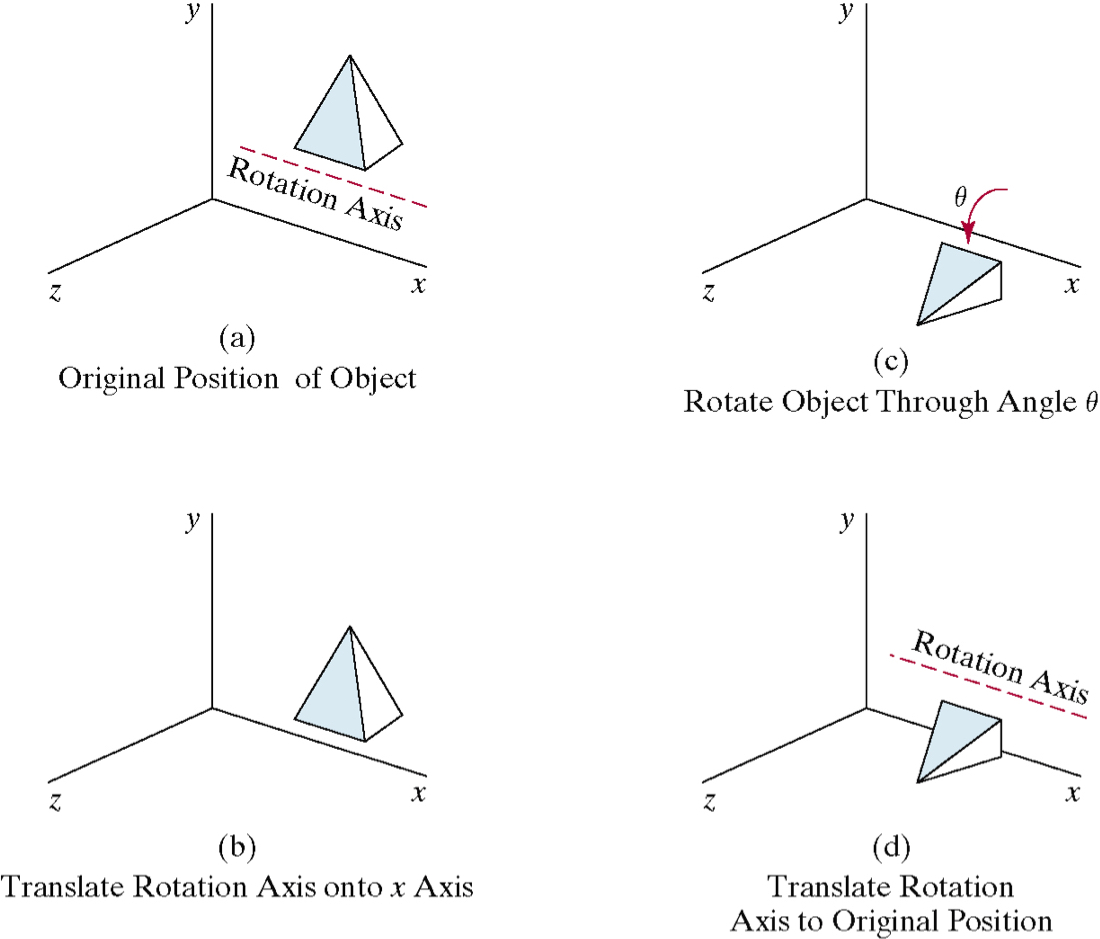
\includegraphics[width=\columnwidth]{general-3d-rotation-1.jpeg}
\end{figure}
좌표축이 아니라 임의의 축을 중심으로 회전하는 경우. 점 $P$를 좌표축으로 옮기고, 회전한 뒤 원래 자리로 옮겨놓는다.
$$
P^\prime = T^{-1} \cdot R_x(\theta) \cdot T \cdot P
R(\theta) = T^{-1} \cdot R_x(\theta) \cdot T
$$
축이 아니라 임의의 방향으로 회전하는 경우. 가령 $P_2$를 $P_1$ 기준으로 회전하는 경우.
\begin{figure}[h]
  \centering
  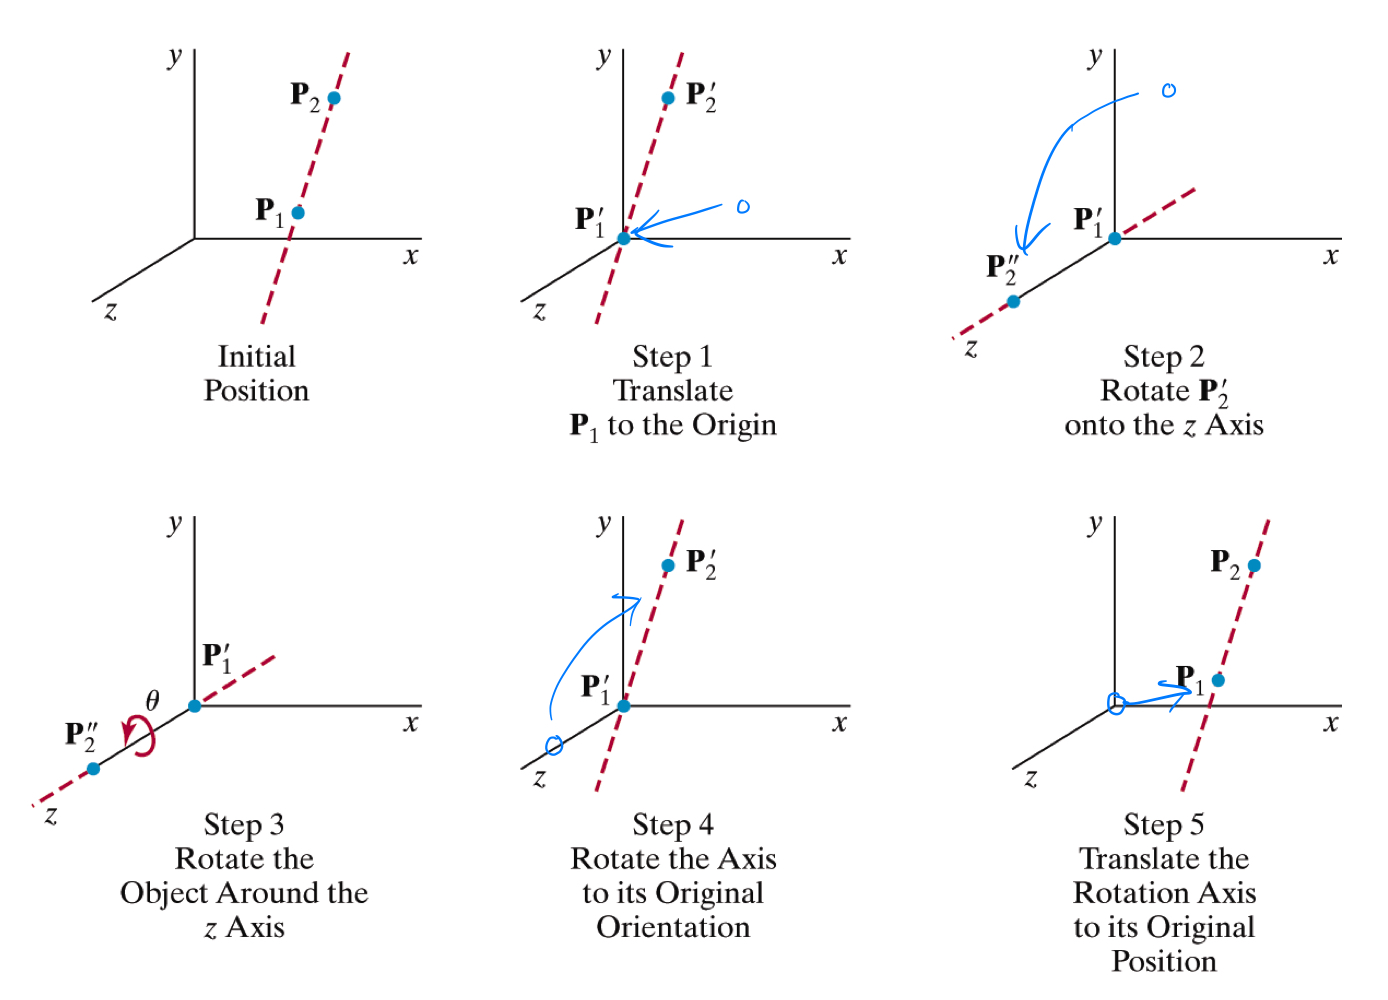
\includegraphics[width=\columnwidth]{general-3d-rotation-2.jpeg}
\end{figure}

\subsection{3D Scailing}

원점을 중심으로 크기 변환하는 경우.
$$
\begin{aligned}
  P^\prime &= S \cdot P \\
  \begin{bmatrix}
    x^\prime \\
    y^\prime \\
    z^\prime \\
    1
  \end{bmatrix}
  &=
  \begin{bmatrix}
    s_x & 0 & 0 & 0 \\
    0 & s_y & 0 & 0 \\
    0 & 0 & s_z & 0 \\
    0 & 0 & 0 & 1
  \end{bmatrix}
  \begin{bmatrix}
    x \\
    y \\
    z \\
    1
  \end{bmatrix}
\end{aligned}
$$
원점이 아니라 고정점을 중심으로 변환하는 경우에는 원점으로 이동, 변환, 다시 제자리로 이동.
$$
\begin{aligned}
  T(x_f, y_f, z_f) \cdot S(s_x, s_y, s_z) \cdot T(-x_f, -y_f, -z_f) \\
  =
  \begin{bmatrix}
    s_x & 0 & 0 & (1 - s_x)x_f \\
    0 & s_y & 0 & (1 - s_y)y_f \\
    0 & 0 & s_z & (1 - s_z)z_f \\
    0 & 0 & 0 & 1
  \end{bmatrix}
\end{aligned}
$$

\section{Viewing}

3차원 월드에서 카메라의 시점.

\subsection{3D Viewing Pipeline}

\begin{figure}[h]
  \centering
  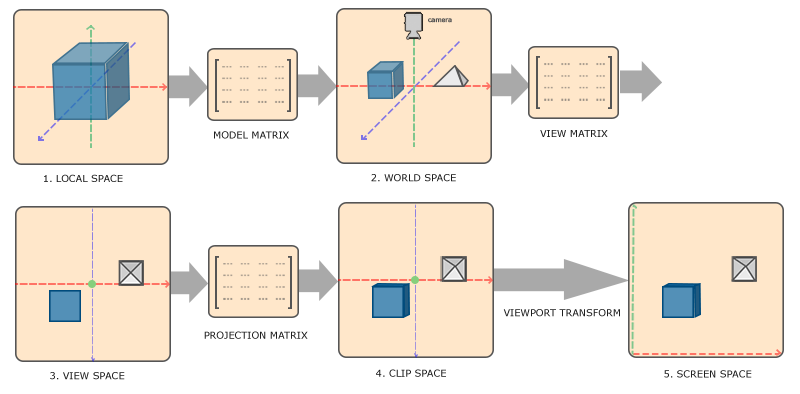
\includegraphics[width=\columnwidth]{viewing-pipeline.png}
\end{figure}

\begin{enumerate}
  \item \textbf{Model Coordinates}: 개별 개체의 좌표계.
  \item Modeling Transform: 모델을 원하는 위치에 배치.
  \item \textbf{World Coordinates}: 개별 개체가 통합된 세계의 좌표계.
  \item Viewing Transform: 월드 좌표계를 카메라 중심으로 조정.
  \item \textbf{Viewing(Camera) Coordinates}: 카메라로 보는 좌표계.
  \item Projection/Normalize Transform: 좌표계 정규화, 원근감 표현.
  \item \textbf{Normalized Coordinates}: -1에서 1 사이 값을 갖는 표준화된 좌표계.
  \item Viewport Transform: 정규화된 좌표를 출력 장치 좌표계에 실제 화면 좌표로 2D 매핑.
  \item \textbf{Screen Coordinates}: 화면의 좌표계.
\end{enumerate}

\subsection{Viewing Coordinate Params}

뷰잉 좌표계는 카메라의 위치, 방향, 위쪽 방향에 따라 설정된다. 카메라의 위치 $P_0$, 카메라의 up vector, 카메라의 방향(-z). 이때 점 $P_{ref}$를 바라본다고 가정.
\begin{figure}[h]
  \centering
  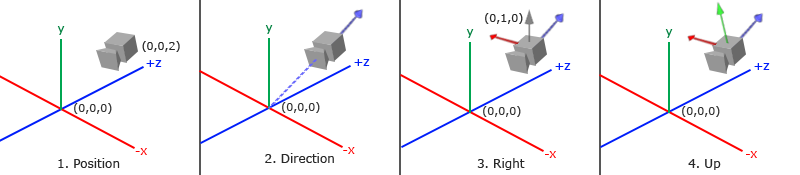
\includegraphics[width=\columnwidth]{camera-axes.png}
\end{figure}
\textbf{normal vector} $n$ ($z_\text{view}$): 카메라가 바라보는 방향. 카메라의 위치 $P_0$에서 카메라가 바라보는 대상의 위치 $P_\text{ref}$를 빼면 얻을 수 있다. 카메라는 z축의 음의 방향을 가리키고 있다.
$$
N = P_0 - P_\text{ref}, \quad \therefore n = {N \over |N|}
$$
\textbf{up vector} $v$ ($y_\text{view}$): 카메라의 위쪽 축. 사용자가 지정한 $V^\prime$에 따라 결정된다.
$$
\begin{aligned}
  V^\prime &= (V^\prime \cdot n)n + V \\
  V &= V^\prime - (V^\prime \cdot n)n \quad \therefore v &= {V \over |V|}
\end{aligned}
$$
\textbf{right vector} $u$ ($x_\text{view}$): 카메라의 오른쪽 축.
$$
u = v \times n
$$

\subsection{Viewing Transformation (WC-VC)}

월드 좌표계를 카메라 좌표 $P_0 = (x_0, y_0, z_0)$를 중심으로 조정하는 변환. $T$로 좌표계의 원점을 카메라의 원점으로 옮기고, $R$로 회전시킨다.
$$
\begin{aligned}
  T =
  \begin{bmatrix}
    1 & 0 & 0 & -x_0 \\
    0 & 1 & 0 & -y_0 \\
    0 & 0 & 1 & -z_0 \\
    0 & 0 & 0 & 1
  \end{bmatrix}
  &\quad
  R =
  \begin{bmatrix}
    u_x & u_y & u_z & 0 \\
    v_x & v_y & v_z & 0 \\
    n_x & n_y & n_z & 0 \\
    0 & 0 & 0 & 1
  \end{bmatrix} \\
  M_{WC, VC} &= R \cdot T
\end{aligned}
$$

\subsection{Projection/Normalize Transformation (VC-NC)}

가상의 평면에 개체를 투영(projection)할 때 투영 방식을 선택해 변환할 수 있음.
\begin{itemize}
  \item Parallel projection: 평행선을 따라 투영하는 것. 개체를 구성하는 모든 점에 대해 투영 방향이 평행하다. 원근법이 반영되지 않기 때문에 있는 그대로의 길이를 측정할 때 쓴다. 어느 방향으로 투영할지에 대한 정보만 있으면 된다: Direction of projection(DOP)
  \item Perspective projection: 소실선을 따라 투영하는 것. 원근감이 적용된다.
\end{itemize}

\subsubsection{Orthogonal Projection}

직육면체를 view volume으로 사용하는 projetion. view volume의 near와 far의 크기가 동일하기 때문에 원근감이 적용되지 않는다.
$$
\begin{bmatrix}
  x^\prime \\
  y^\prime \\
  z^\prime \\
  1
\end{bmatrix}
=
\begin{bmatrix}
  1 & 0 & 0 & 0 \\
  0 & 1 & 0 & 0 \\
  0 & 0 & 0 & 0 \\
  0 & 0 & 0 & 1
\end{bmatrix}
\begin{bmatrix}
  x \\
  y \\
  z \\
  1
\end{bmatrix}
$$
아래 나오는 normalize를 한 다음 위 projection을 적용하면 된다.

\subsubsection{Clipping Window \& View Volume}

clipping window는 view plane 앞에 놓인 윈도우. 밖에 있는 개체가 잘린다(clipping).
\begin{figure}[h]
  \centering
  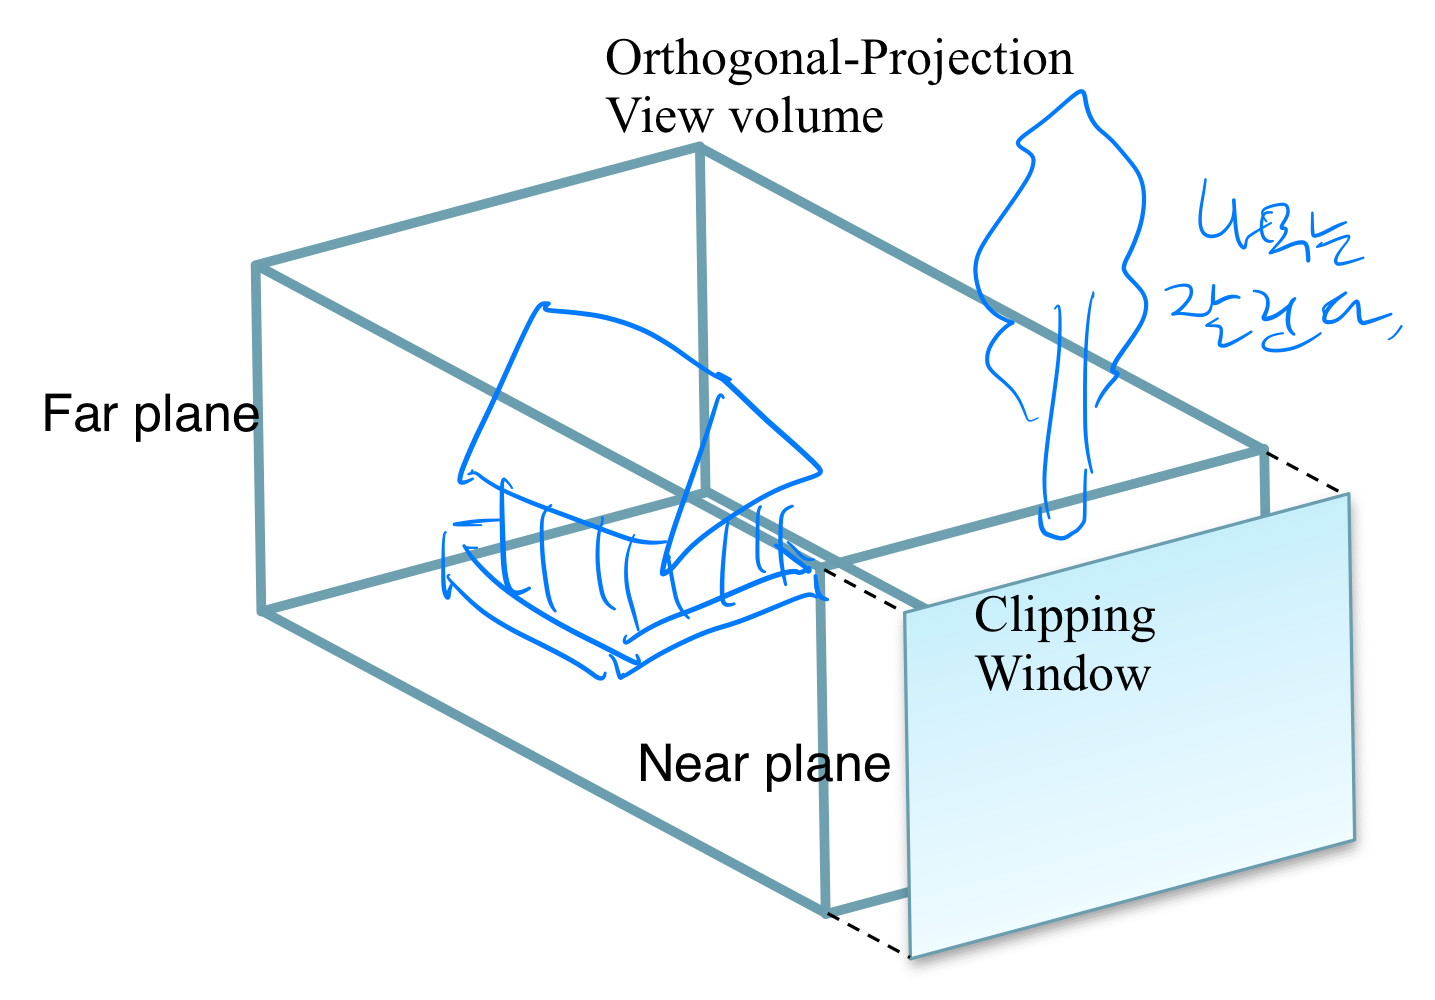
\includegraphics[width=70mm]{orthogonal-projection-view-volume.png}
\end{figure}
clipping volume은 far plane과 near plane을 정의해 멀리있는 물체가 잘리게 된다.

\subsubsection{Normalized View Volume}

x, y, z 좌표는 각각 0에서 1 또는 -1에서 1 범위로 정규화된다. orthogonal한 박스에 넣는 것. 이는 장치에서 독립적인 좌표다.
$$
\begin{aligned}
  w &=  x_\text{max} - x_\text{min} \\
  y &= y_\text{max} - y_\text{min} \\
  d &= z_\text{near} - z_\text{far} \\
  M_{ortho, norm} &=
  \begin{bmatrix}
    {2 \over w} & 0 & 0 & -{x_\text{max} + x_\text{min} \over w} \\
    0 & {2 \over h} & 0 & -{y_\text{max} + y_\text{min} \over h} \\
    0 & 0 & {2 \over d} & {z_\text{near} + z_\text{far} \over d} \\
    0 & 0 & 0 & 1
  \end{bmatrix}
\end{aligned}
$$
$M_{ortho, norm}$는 orthographic projections를 normalized 좌표로 변환한다.
\begin{figure}[h]
  \centering
  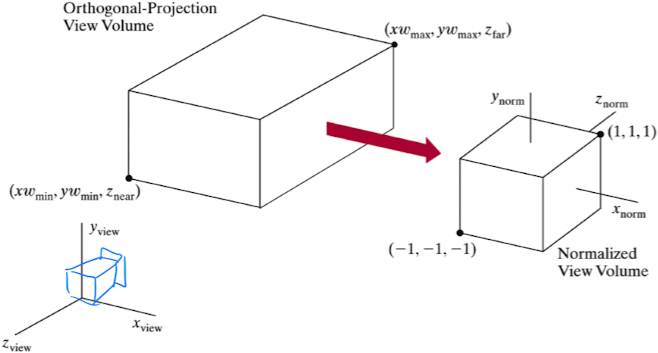
\includegraphics[width=\columnwidth]{orthogonal-normalized.png}
\end{figure}
oblique projection은 DOP를 비스듬하게 만든 것.

\subsubsection{Perspective Projection}

절두체를 view volume으로 사용하는 projection. 삼각형의 닮음비를 이용해 변환할 수 있다.
\begin{figure}[h]
  \centering
  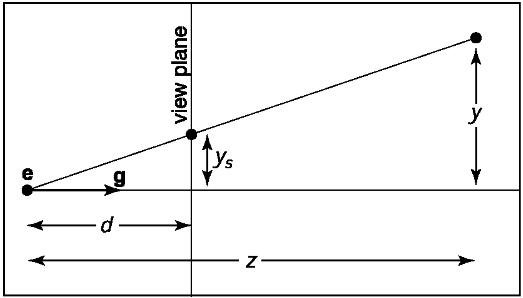
\includegraphics[width=\columnwidth]{perspective-projection.png}
\end{figure}
이때 $y_s = d {y \over z}$.
$$
\begin{aligned}
  M_{\text{perspective}} =
  \begin{bmatrix}
    1 & 0 & 0 & 0 \\
    0 & 1 & 0 & 0 \\
    0 & 0 & 1 & 0 \\
    0 & 0 & 1/d & 0
  \end{bmatrix}
  \text{or}
  \begin{bmatrix}
    d & 0 & 0 & 0 \\
    0 & d & 0 & 0 \\
    0 & 0 & d & 0 \\
    0 & 0 & 1 & 0
  \end{bmatrix}
\end{aligned}
$$
3차원 좌표에 $M_{\text{perspective}}$를 곱하면 원근감이 적용된다. 만약 $(x, y, z, 1)$에 적용하면 $(x, y, z, {z \over d})$가 되고, 이를 cartesian coordinate로 바꾸면 $(x{d \over z}, y{d \over z}, d)$. 따라서 거리 d가 멀어질수록 작아보이는 것. 여기서 homogeneous coordinate를 써야 하는 이유를 또 하나 발견. 마지막 row를 이용해 나눗셈을 할 수 있음.

만약 어떤 크기 변환 $s_z$와 이동 변환 $t_z$가 있을 때 perspective projection을 적용한다면:
$$
\begin{aligned}
  \begin{bmatrix}
    x^\prime \\
    y^\prime \\
    z^\prime \\
    1
  \end{bmatrix}
  &=
  \begin{bmatrix}
    d & 0 & 0 & 0 \\
    0 & d & 0 & 0 \\
    0 & 0 & s_z & t_z \\
    0 & 0 & 1 & 0
  \end{bmatrix}
  \begin{bmatrix}
    x \\
    y \\
    z \\
    1
  \end{bmatrix} \\
  &=
  \begin{bmatrix}
    dx \\
    dy \\
    s_zz + t_z \\
    z
  \end{bmatrix}
  =
  \begin{bmatrix}
    dx \over z \\
    dy \over z \\
    s_z + {t_z \over z} \\
    1
  \end{bmatrix} \\
  &= ({x \over z / d}, {y \over z / d}, s_z + {t_z \over z})
\end{aligned}
$$
카메라 중심으로 변환했으므로 모든 대상물이 -z 축에 있음. z값은 음수일 때, $[-z_\text{near}, -z_{far}]$를 $[-1, 1]$로 normalize하고 싶다면:
$$
\begin{aligned}
  A &= -{z_\text{far} + z_\text{near} \over z_\text{far} - z_\text{near}} \\
  B &= -{2z_\text{far} z_\text{near} \over z_\text{far} - z_\text{near}} \\
  \begin{bmatrix}
    x^\prime \\
    y^\prime \\
    z^\prime \\
    1
  \end{bmatrix}
  &=
  \begin{bmatrix}
    z_\text{near} & 0 & 0 & 0 \\
    0 & z_\text{near} & 0 & 0 \\
    0 & 0 & A & B \\
    0 & 0 & -1 & 0
  \end{bmatrix}
  \begin{bmatrix}
    x \\
    y \\
    z \\
    1
  \end{bmatrix} \\
  &=
  \begin{bmatrix}
    z_\text{near}x \\
    z_\text{near}y \\
    Az + B \\
    -z
  \end{bmatrix}
  =
  \begin{bmatrix}
    z_\text{near}x \over -z \\
    z_\text{near}y \over -z \\
    -A - {B \over z} \\
    1
  \end{bmatrix}
\end{aligned}
$$
여기서 주목할 점은 마지막 행의 세 번째 열에 $-1$이 들어갔다는 점. perspetive projection을 적용한다.

\subsection{Viewport Transformation (NC-SC)}

normalized coordinates를 screen coordinates로 변환. 우선 view volume을 viewport의 width와 height에 맞게 크기를 변환한다. view port가 $(x_\text{min}, y_\text{min})$와 $(x_\text{max}, y_\text{max})$로 정의된 사각형이라면, width $w = x_\text{max} - x_\text{min}$, height $h = y_\text{max} - y_\text{min}$.
$$
\hat S =
  \begin{bmatrix}
    w \over 2 & 0 & 0 & 0 \\
    0 & h \over 2 & 0 & 0 \\
    0 & 0 & 1 \over 2 & 0 \\
    0 & 0 & 0 & 1
  \end{bmatrix}
$$
크기 변환 후에는 view volume을 viewport의 원점$({w \over 2}, {h \over 2})$을 기준으로 오프셋 $x_\text{min}, y_\text{min}$만큼 이동한 위치에 배치한다.
$$
\hat T =
  \begin{bmatrix}
    1 & 0 & 0 & {x_\text{max} + x_\text{min} \over 2} \\
    0 & 1 & 0 & {y_\text{max} + y_\text{min} \over 2} \\
    0 & 0 & 1 & 1 \over 2 \\
    0 & 0 & 0 & 1
  \end{bmatrix}
$$
따라서,
$$
M_\text{NC, SC} =
\hat T \hat S =
  \begin{bmatrix}
    w \over 2 & 0 & 0 & {x_\text{max} + x_\text{min} \over 2} \\
    0 & h \over 2 & 0 & {y_\text{max} + y_\text{min} \over 2} \\
    0 & 0 & 1 \over 2 & \over 2 \\
    0 & 0 & 0 & 1
  \end{bmatrix}
$$

이때  w를 스크린의 width pixel 개수, h를 스크린의 height pixel 개수로 생각해도 된다.

\section{Rasterization}

\begin{itemize}
  \item Scan conversion: 몇 개의 픽셀을 선택해 표현할지 고르는 과정. 프래그먼트의 집합을 만들어낸다. 프래그먼트는 픽셀과 일대일 대응이 아닐 수 있다.
  \item DDA(Digital Differential Analyzer) Algorithm: 개체를 포함하는 픽셀을 칠하는 방식. x축을 기준으로 y 좌표를 포함하는 픽셀을 칠한다. 기울기가 1보다 크면 끊겨 보이기 때문에 y축을 기준으로 그린다.
  \item Bresenham's Algorithm: flaot point 연산에 비용이 많이 들기 때문에 고안된 방법. 요즘에는 컴퓨터 성능이 좋기 때문에 scan conversion하면 된다.
\end{itemize}

\subsection{Polygon Scan Conversion}

winding number를 이용해 칠해야할 영역을 찾는 방식. 개체 밖에서 개체를 관통하는 수평선을 그렸을 때 볼록 다각형은 항상 두 지점에서 수평선과 맞닿는다. 이때 y가 증가하는 부분에서는 winding nubmer를 1 증가시키고, 감소하는 부분에서는 1 감소시켜 그 값이 $n$인 부분만 칠한다.
\begin{figure}[h]
  \centering
  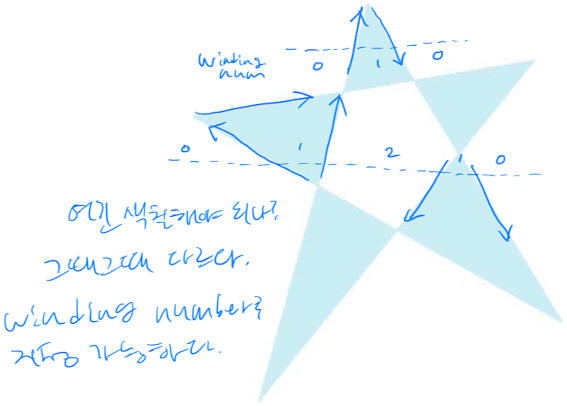
\includegraphics[width=\columnwidth]{polygon-scan-conversion.png}
\end{figure}
홀수일때만 채우거나, 0이 아닐때만 채우도록 할 수도 있기 때문에 odd-even fill이라고 함.

만약 칠하려는 개체가 만약 볼록 다각형이 아니라면 문제가 생긴다. 무조건 convex하게 만들기 위해 한 개체를 여러 개의 삼각형으로 쪼갠다. 이걸 tessellation이라고 한다.
\begin{figure}[h]
  \centering
  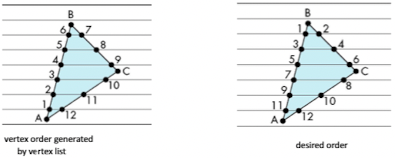
\includegraphics[width=\columnwidth]{scan-line-fill.png}
\end{figure}
개체를 관통하는 가상의 sacn lines를 그린다. 이때 scan line의 두 교점 사이를 칠하는 방식.

각 정점의 색깔을 다르게 칠할 수도 있음. 삼각형의 꼭짓점 A, B, C의 색이 주어졌을 때 임지의 점 T의 색은 내분점으로 interpolate해서 구할 수 있다.

\subsection{Polygon Aliasing}

개체에 비해 픽셀이 너무 큰 경우 문제가 됨. 샘플링이 부족해서 생기는 모든 문제를 aliasing이라고 한다. 레티나 디스플레이는 25cm 정도 떨어진 위치에서 화면을 봤을 때 aliasing 문제가 생기지 않을 정도의 해상도.

\subsection{Anti-aliasing by Area Averaging}

개체가 픽셀을 차지한 비율만큼 색을 칠하면 aliasing 문제를 해결할 수 있다(area averaging). 근데 다른 방법도 있다.

\begin{itemize}
  \item Supersampling: 각 픽셀에 대해 여러 점을 샘플링해서 색상의 평균을 낸다. fragment shader를 여러 번 돌리는 셈.
  \item Multisampling: 평면까지 샘플링할 필요는 없다는 발상. 개체의 외각선이 지나가는 곳, 즉, 경계 부분에서만 샘플링한다.
\end{itemize}

\section{Visibility}

개체가 실제로 앞에 있는지, 뒤에 있는지와 상관없이 렌더링을 마지막에 한 개체가 위에 보이는 문제. 간단히 뒤에 있는 개체를 먼저 그릴 수도 있지만, cyclic overlap, penetration 같은 경우에는 해결이 안 됨.

\subsection{Back-Face Removal (Culling)}

개체의 뒷면은 안 보이니까 그리지 않아도 된다. 그렇다면 어디가 앞인지 알아야 함. 이때 개체의 normal vector 구하면 된다. normal vector가 -z 축이면 안 그리고, +z 축이면 그린다. 0인 경우 실루엣.

$a \times b = n$인데, $b \times a = -n$이 되는 문제. 정점의 번호가 중요하다. 정면에서 봤을 때 반시계 방향으로 번호를 부여하면 된다.

\subsection{z-buffer Algorithm}

가까운 개체 순서로 그리고, 멀어서 가려지면 렌더링하지 않는 방법. 두 개의 버퍼를 두고 하나는 개체를, 하나는 개체를 구성하는 픽셀별 거리를 저장. 이때 z-buffer(depth buffer)에 카메라로부터 가장 가까운 개체까지의 거리를 저장해둔다. `가까운 물체가 멀리 있는 물체를 가린다'라는 직관적 깊이 개념을 구현하는 것.

\section{Lighting and Shading}

광원으로부터 오는 빛을 물체가 반사하는 것만 표현하는 모델은 local reflection model(local lighting). 개체, 조명, 카메라만 사용한다. 물체가 서로를 반사하는 빛까지 표현하는 global reflection model(global lighting)이 현실적이지만 구현이 어려움. 언리얼 엔진은 local reflection만으로 global reflection을 표현하는 도전.

조명에는 point light, directional light, spot light가 있음. point는 광원 위치에서 물체 위치를 뺀 벡터 $L$이 정점 위치에 의존하는 경우. directional은 $L$이 상수. 광원이 충분히 멀다면 위치보다는 방향이 중요하다.

\subsection{Phong Reflection Model}

반사된 빛 $I$를 아래와 같이 수식으로 표현할 수 있음.
$$
\begin{aligned}
  I = k_aI_a + k_dI_d + k_sI_s \\
  where \quad k_a + k_d + k_s = 1
\end{aligned}
$$
\begin{itemize}
  \item $k_aI_a$: ambient component, 주변광. 수많은 반사를 거쳐 광원이 불분명한 빛. 현실적으로 수많은 빛들의 상호작용을 구현하기 어려워 일정한 밝기와 색으로 근사한다.
  \item $k_dI_d$: diffuse component, 분산광. 물체의 표면에서 분산되는 빛. 각도에 따라 밝기가 달라진다.
  \item $k_sI_s$: specular component, 반사광. 분산광과 달리 한 방향으로 완전히 반사되는 빛. 반사되는 부분이 흰색으로 반짝여 보인다.
\end{itemize}

\subsubsection{Diffuse reflection (Lambertian)}

$$
I_d  = I_i \cos{\theta} = I_i(L \cdot N)
$$

빛이 닿는 면의 경사도에 따라 단위 면적당 빛이 적어짐. 기울기가 점점 기울어져 음수가 되면 0으로 한계를 설정해야 한다.

\begin{itemize}
  \item $I_i$: indensity of incident light.
  \item $L$: 빛의 방향 (unit)
  \item $N$: 점에서의 법선. 빛이 들어오는 양이 $N$에 따라 달라짐. (unit)
  \item $\theta$: $N$과 $L$ 사이의 각.
\end{itemize}

$N$과 $L$ 만으로 반사되는 빛의 양을 계산하는 것. $N$과 $L$이 unit vector라면 $\cos \theta = N \cdot L$.

\subsubsection{Specular component}

$$
I_s = I_i\cos^n{\Omega} = I_i(R \cdot V)^n
$$

보는 방향 $V$와 빛이 반사되는 방향 $R$이 일치하면 반짝여보임.

\begin{itemize}
  \item $V$: viewing direction (unit)
  \item $R$: reflection direction (unit)
  \item $\Omega$: $V$와 $R$ 사이의 각.
  \item $n$: $\cos^n$에서 $n$이 커질수록 뾰족한 그래프가 만들어진다. 각이 좁아질수록($n$이 클수록) 더 좁은 영역이 더욱 반짝임. 이때 $n$이 shininess.
\end{itemize}

$N$과 $L$을 알면 $R$을 구할 수 있다: $R = 2(L \cdot N)N - L$.

\subsubsection{Final Phong Reflection}

$$
I = k_aI_a + I_i(k_d(L \cdot N) + k_s(R \cdot V)^n)
$$

$k_d$(알베도)는 물체의 색깔. $k_s$는 항상 흰색. 금속의 경우 $k_s$는 표면의 색상으로, $k_d$는 0으로 하면 된다.

\subsection{Blinn-Phong Model}

Phong 모델의 floating point 연산을 피하기 위한 모델. $H$는 $L$과 $V$의 중간에 있는 halfway 벡터($(L + V) / 2$)인데, 만약 $V$가 $L$의 반사 벡터인 $R$에 있다면 $H$는 $N$과 같아진다. 따라서 $R \cdot V$ 대신 $N \cdot H$를 쓸 수 있다.

이때 멀리있는 광원 $L$은 고정되어 있고, $V$도 카메라가 충분히 멀다면 그냥 z 방향이라고 취급할 수 있음. 결과적으로 $H$를 상수로 만듦으로써 픽셀마다 빛을 계산하던 연산을 줄일 수 있다. 사실 미묘하게 결과가 달라서 잘못된 모델이지만 레거시라서 제공은 된다.

\subsection{Flat \& Gouraud Shading}

lighting은 물체와 조명간의 상호작용으로 물체가 빛을 어떻게 반사하는지 계산하는 것. shading은 라이팅을 했을 때 물체의 색깔을 결정하는 것.

Flat은 lighting 계산을 면마다 한번만 하는 shading 방식. 구를 못 만들어서 면으로 이어붙인건데 면 하나를 통째로 같은 명암으로 설정하는건 취지에 맞지 않으므로 잘못된 방식.

Gouraud는 lighting을 삼각형의 꼭짓점마다 한번만 계산하는 방식. 정점 주변 4개 면의 normal을 모두 더해서 그 개수로 나눈 평균값을 해당 정점의 normal로 사용. 연산량이 줄어들지만 어색.

\subsection{Phong Shading}

\begin{figure}[h]
  \centering
  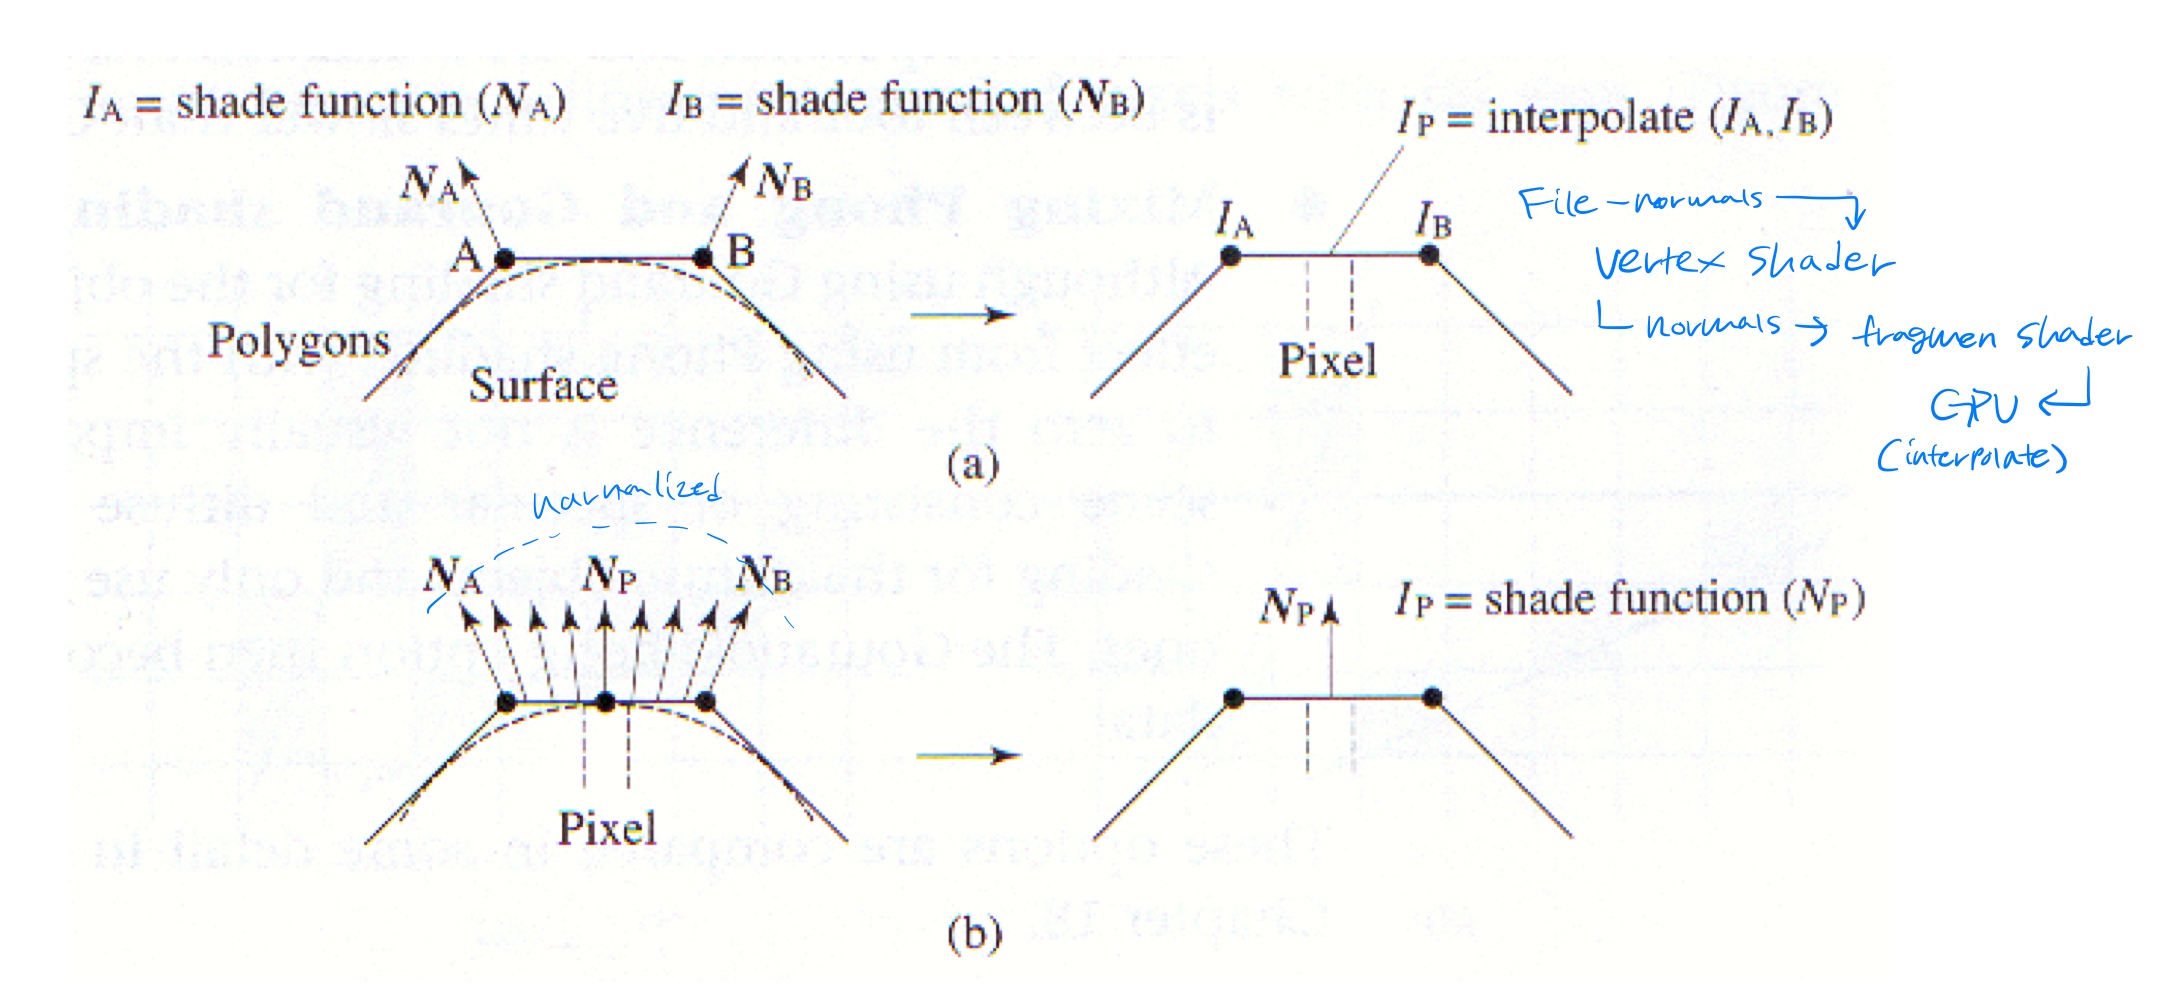
\includegraphics[width=\columnwidth]{phong-shading.jpeg}
\end{figure}

어떤 면이 주어졌을 때 디자이너의 의도는 곡면이었을 것이라는 추측 가능. 한 도형에서도 각 정점의 normal이 다르기 때문에 Phong shading은 정점마다 normal을 보간한다. 각 점의 normal을 구하고 normalize하면 길이가 맞춰짐.

\subsection{sRGB vs Linear}

모니터에 색상을 0으로 주면 검은색, 1로 주면 흰색이 나올 것. 0.5라면? 회색이 나오긴 하지만, 실제 중간값이 아니라 훨씬 어두운 색상이 나옴. 에너지 값을 그래픽 카드에 보냈을 때 그대로 빛으로 바꿔주지 않기 때문. 해결하려면 모니터에 걸리는 전압, 그 에너지 값을 고려해 모니터의 색상값으로 바꾸는 과정이 필요, 그 표준이 sRGB.

\subsection{Advanced Rendering}

실제 세상에서 빛의 반사는 반구 $\Omega$에 들어오는 빛 $\omega_i$가 점 $x$에서 반사해 $\omega_o$ 방향으로 나간다. 아래는 $L_o$, 즉 $t$ 시점에 $\lambda$ 파장으로 점 $x$에서 반사되어 $w_o$로 들어오는 빛을 구하는 식.
$$
\begin{aligned}
  L_o(x, \omega_o, \lambda, t) = L_e(x, \omega_o, \lambda, t) + \\
  \int_\Omega f_r(x, \omega_i, \omega_o, \lambda, t)L_i(x, \omega_i, \lambda, t)(\omega_i \cdot n)d\omega_i
\end{aligned}
$$
여기서 $f_r$은 반사율. BRDF(Bidirectional Reflectance Distribution Function)라고 한다. 실제 물질의 빛 반사를 실측한 값을 사용한다. 이때 물체를 돌려도 빛이 동일한 것은 isotropic, CD처럼 돌리면 빛이 변하는 것은 anisotropic.

디자이너가 실측하기 어려우므로 BRDF를 근사하도록 만들어뒀다.

\section{Texture Mapping}

텍스처 매핑은 텍스처 이미지를 3D 개체 표면에 매핑하는 것. window 좌표계의 특정 점을 world 좌표계에서 찾고, 그것을 parametric 좌표계에서 찾고, 그것을 또 texture 좌표계에서 찾아야 한다. 몇가지 mapping 방법이 있음.

\begin{itemize}
  \item Planar: X-Y 좌표계를 텍스처 좌표계로 대응. 하지만 z축으로 깊어지면 텍스처가 그냥 늘려짐.
  \item Spherical \& Cylindrical \& Box: 구, 원통, 박스에 매핑하는 방식. 다 문제가 있음. cylinder의 경우 위에서 보면 planar와 같은 문제.
\end{itemize}

실제로는 디자인 단계에서 3D 개체에 2차원 텍스처 좌표를 저장해둔다.

\subsection{Diffuse map}

개체의 표면의 색상을 정의하는 텍스처. vertex마다 위치와 색깔을 설정할 수는 있지만, vertex를 너무 잘게 쪼개야 하기 때문에 텍스처를 사용함. vertex shader에서 fragment shader로 vertex 정보를 전달할 때 GPU가 interpolation을 해 지정한 슬롯의 텍스처에서 지정된 픽셀 색상을 가져오게 된다.

\subsection{Bump map (normal map)}

개체 표면의 울퉁불퉁함을 정의하는 텍스처. original surface의 geometry를 조작하는 것이 아니라, 반사되는 빛을 조정하는 것. 홈이 파인 부분이 너무 어둡게 나오기 때문에 어느정도로 어두워야 하는지 설정하기 위해 ambient occlusion map을 사용할 수도.

\subsection{Aliasing Problem}

텍스처의 픽셀을 텍셀이라고 부름. 원근법이 적용된 상태에서 멀리있는 픽셀의 텍스처를 가져오기 위해 해당하는 텍셀을 선택하면 너무 넓은 면적의 텍셀이 선택되는 문제가 있다.

샘플링을 많이 해도 되긴 하지만, 상대적으로 거대한 텍셀에서 몇 개 더 샘플링한다고 큰 차이가 없음. 다른 방법은 텍셀을 평균낸 값을 가져오는 것. 하지만 매번 평균을 내면 연산이 너무 많다. 그 해결책은 Mip-Mapping. 큰 텍스처의 여러 영역을 평균내어 작은 버전의 텍스처를 미리 만들어 두는 것. 작은 개체의 텍스처를 작은 텍스처에서 가져오면 된다.

\subsection{Anisotropic Filtering}

텍스처가 뿌옇게 보이는 문제. 텍스처를 x로만 줄인 버전, y로만 줄인 버전, xy 모두 줄인 버전을 모두 만들어두고 사용하면 된다.

\section{Shadows and Multi-Pass Rendering}

빛을 가려 그림자를 만드는 개체는 Creator. 그림자가 비춰지는 개체는 Reciever. 한 개체가 creator이자 receiver일 수 있다. point source는 딱 떨어지는 umbra를 형성하지만, 광원의 크기가 커져 area source가 되면 softshadow가 일어나는 penumbra가 함께 형성된다.

어떻게 그림자를 표현할까? 그림자 텍스쳐를 입힐 수도 있음(baking). 하지만 조명과 물체를 움직일 수가 없다.

\subsection{Shadow Volume}

creator로 빛이 가려지면 뒤쪽의 절두체 볼륨이 그림자라고 간주할 수 있음. 카메라 시점에서 shadow volume 면이 먼저 보이면 그림자 안에 있다고 판단. 지금은 안 쓰임.

\subsection{Shadow Mapping}

빛의 위치에서 월드를 봤을 때 안 보이는 부분을 그림자로 간주. 이때 빛에서 각 픽셀까지의 depth를 프레임 버퍼 오브젝트에 저장해둔다. 다만 이렇게 만든 shadow depth map은 사용자에게 보이지 않게 렌더링한다. 이렇게 화면에 그리지 않는 렌더링은 off-screen rendering.

\begin{figure}[h]
  \centering
  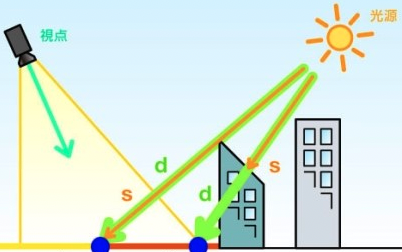
\includegraphics[width=\columnwidth]{shadow-mapping.png}
\end{figure}

카메라가 어떤 점을 봤을 때, 해당 픽셀과 광원의 거리가 shadow map의 해당 픽셀에 쓰여진 광원과 creator의 거리보다 크다면 그림자. 즉, shadow map에 카메라가 보는 픽셀의 depth가 아니라 다른 픽셀의 depth가 쓰여 있다면 그림자로 간주.

빛 위치에서 세상을 보려면 새로운 view projection matrix를 만들어야 한다. (MVP: Model View Projection) 카메라가 보는 픽셀을 shadow map의 픽셀에 대응시킬 때도 MVP가 필요하다. 이때 shadow map의 projection은 orthogonal이다.

\subsection{Shadow Acne}

그림자가 없어야 하는 곳에 나타나는 그림자 무늬. shadow map의 해상도가 무한하지 않으므로 shadow map은 픽셀을 샘플링해 구성된다. 그런데 샘플링의 오차로 인해 shadow map의 텍셀 기준으로 특정 픽셀의 그림자를 판정하려 할 때, 실제로는 자신을 가리는 개체가 없음에도 참조한 shadow map의 텍셀에는 자신을 가리는 다른 픽셀의 depth가 저장되어 있는 케이스가 발생한다. 때문에 필연적으로 shadow acne가 나타난다.

shadow map에 bias를 적용해 depth를 미세하게 조정하면 해결할 수 있다. 하지만 bias가 너무 크면 개체로부터 그림자가 분리되는 peterpanning이 일어난다. 따라서 bias를 적절히 설정하거나, shadow acne를 가리도록 개체의 위치나 두께 등을 조정해야 한다.

\subsection{Shadow Aliasing}

그림자 경계 부분이 계단처럼 울퉁불퉁해 보이는 현상. shadow map을 키워 샘플링을 많이 하면 해결된다. 그게 아니면...

\textbf{Multi sampling (Percentage Closer Filtering)}: poisson distribution에 따라 픽셀을 여러 번 샘플링한다. poisson disk 값이 커지면 그림자의 sharpness가 줄어들어 soft shadow가 표현된다. sharpness가 커져서 날카로워지면 텍셀이 보이는 문제가 생긴다. 이때는 shadow map의 크기를 키울 수 밖에 없다.

\textbf{Percentage-Closer Soft Shadows}: penumbra는 광원의 크기, 빛과 blocker 사이의 거리, 빛과 receiver 사이의 거리에 따른다. 따라서 blocker를 찾고, penumbra의 크기를 계산한다.

\begin{figure}[h]
  \centering
  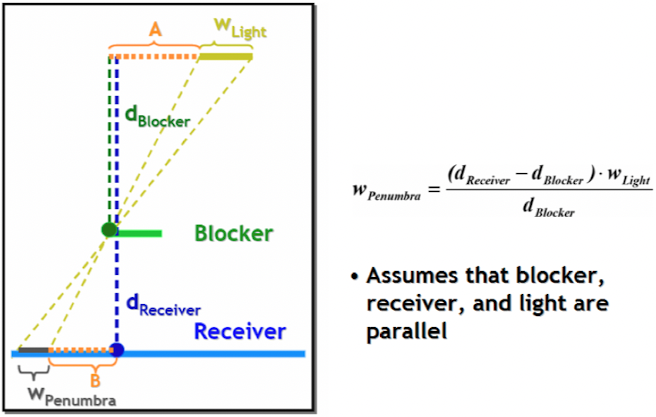
\includegraphics[width=\columnwidth]{penumbra-size.png}
\end{figure}
